\section{Experiments and results}\label{sec:chp6:exp-res}
To evaluate different aspects of the proposed \ac{cad} system, we proposed variety of experiments with respect to individual modalities and their combination. 
Table~\ref{tab:exp-summary} represents the summary of the experiments. 
These experiments and the results obtained are discussed in details in the reminder of this section. 
Pre-processing, segmentation and registration of each modalities are common steps across all the designed experiments.

\subsection{Experiment-1: Assessment of inidivual modalities}\label{subec:chp6:exp-res:Ex1} 
The main goal of this experiment is to eavluate the potential of each inividual modality and their corresponding features. 
Different features as presented in Sect.~\ref{subsec:chp6:method:fea-det} are extracted for different modalities. 
For all the modalities, the extracted features without any extraction or selection process are used to train a \ac{rf} classifier, using a \ac{lopo}. 
These experiments are performed using {\color{red} which dataset}.
The results are presented in terms of \ac{roc} analysis and averaged \ac{auc} over \ac{lopo}.
Figure~\ref{fig:res-Ex1} illustrate the obtained results.

\begin{figure}
  \hspace*{\fill}
  \subfigure[Performance of different pharmacokinetic paramters on \ac{dce}-\ac{mri}]{\label{fig:}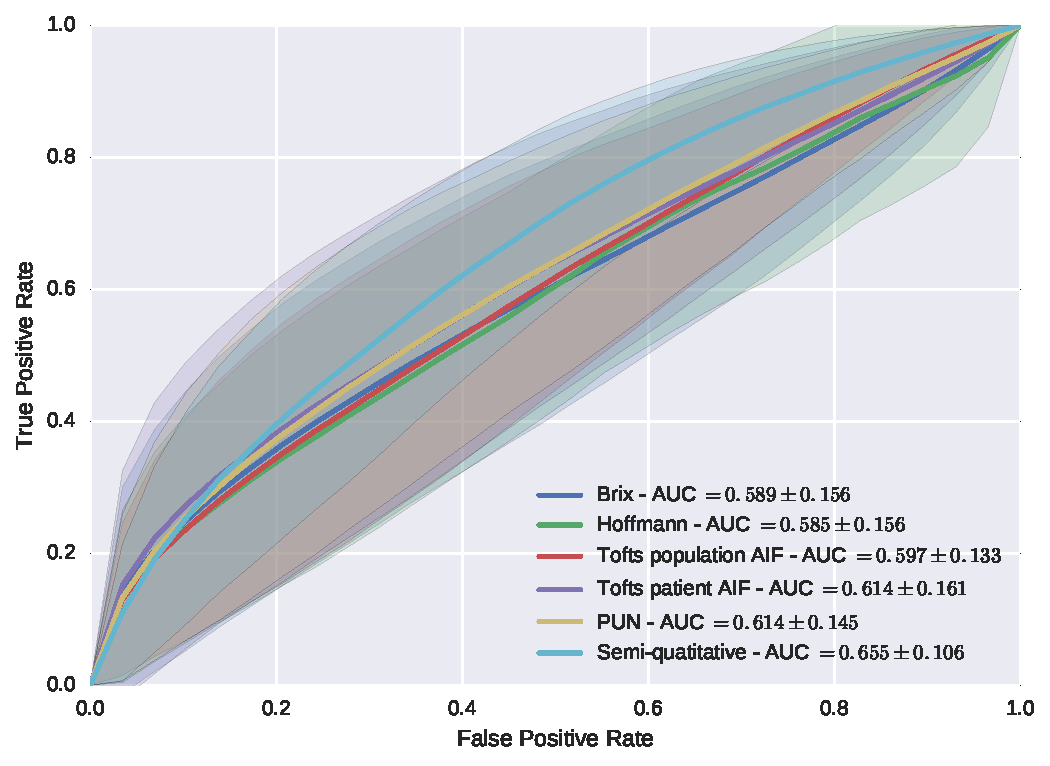
\includegraphics[width=.49\textwidth]{5_normalization/figures/DCE-normalization/normalized_methods_0.pdf}}
  \hfill
  \subfigure[Performance of whole \ac{dce}-\ac{mri} signal]{\label{fig:}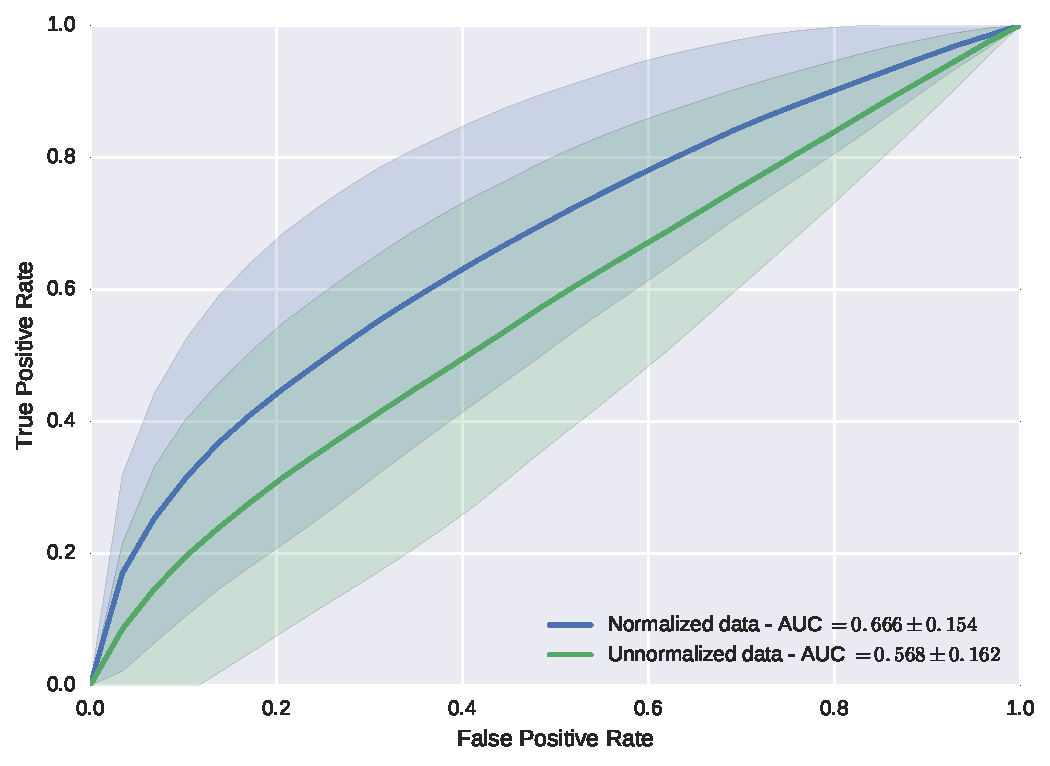
\includegraphics[width=.49\textwidth]{5_normalization/figures/DCE-normalization/full_signal_0.pdf}}
  \hspace*{\fill} \\
  \hspace*{\fill}
  \subfigure[Performance of image-based features for \ac{t2w} and \ac{adc}-\ac{mri}]{\label{fig:}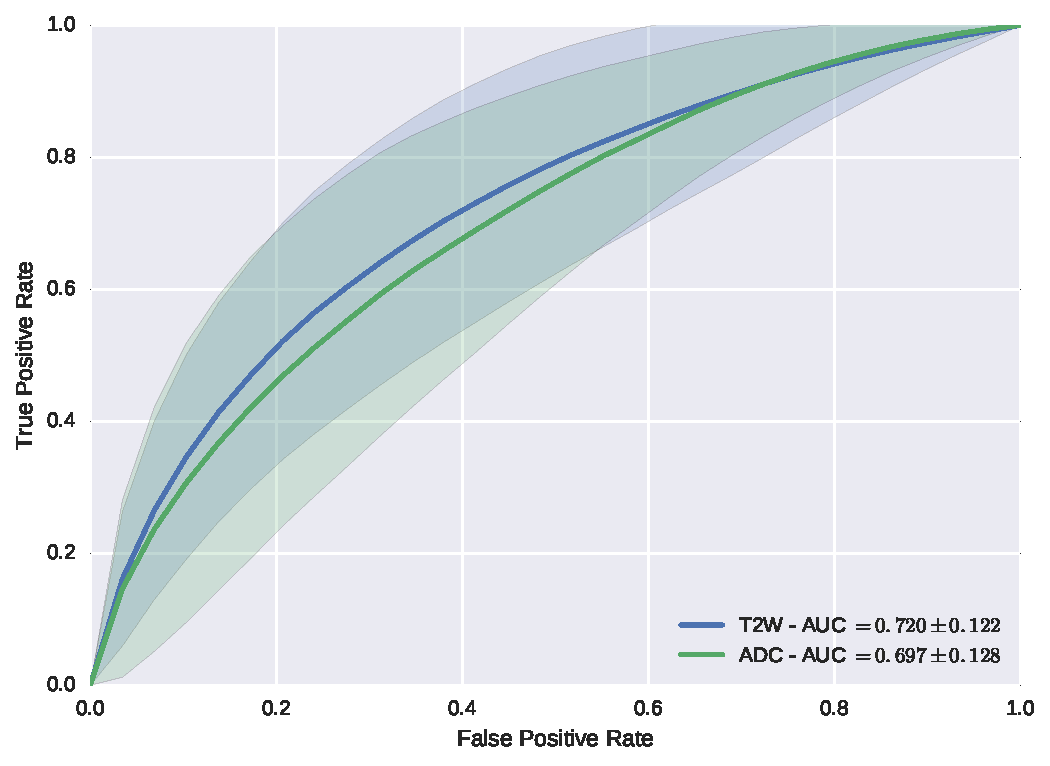
\includegraphics[width=.49\textwidth]{6_pipeline/figures/exp-1/t2w_adc.pdf}}
  \hfill
  \subfigure[Performance of whole spectra using \ac{mrsi} signal]{\label{fig:}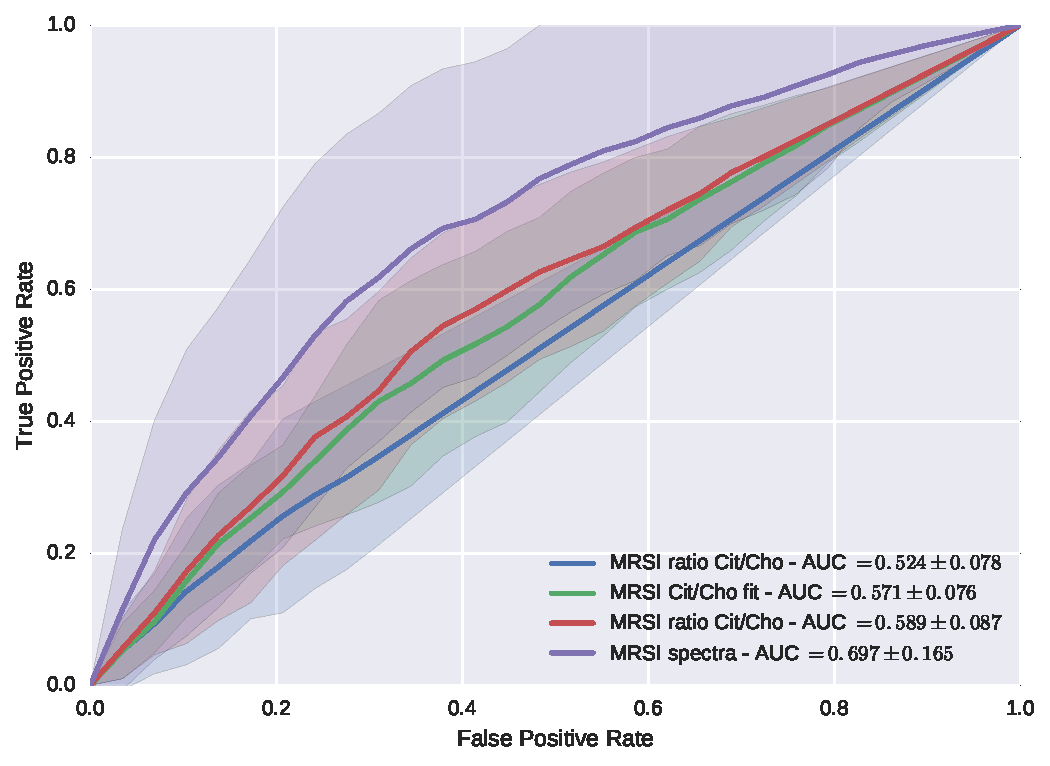
\includegraphics[width=.49\textwidth]{6_pipeline/figures/exp-1/mrsi_all.pdf}}
  \hspace*{\fill}
  \caption[Results obtained from experiment-1]{Results obtained from experiment-1: assessment of inividual modalities}
  \label{fig:res-Ex1}
\end{figure}


\subsection{Experiment-2: Coarse combination} \label{subsec:chp6:exp-res:Ex2}
The objective of this experiment is to evaluate the combination of all the modalities.
To this extent, three different approaches are considered: (i) feature aggregation, (ii) statcking using \ac{adb}, (iii) stacking using \ac{gb}. 
In the first approach, feature aggregation, the features extracted from each modalities (\ac{t2w}, \ac{adc}, normalized-whole-\ac{dce} and normalized-whole-\ac{mrsi}, as concluded in experiment-1) are concatenated together and used with a \ac{rf} classifier and \ac{lopo}. 
In the second and third approach since stacking is used the training set is divided into training and validation set.
Therefore, first a \ac{rf} classifier is trained for each modality using the their corresponding training set and then using a validation set their prediction is fed as a training to a meta learner.
\Ac{adb} and \ac{gb} are used as a meta learner for the second and third approach, respectively. 
Figure~\ref{fig:flow-Ex2} shows the framework of the first and second/third approach. 

The obtained results of this experiment are shown in Fig.~\ref{fig:res-Exp2}.
\begin{figure}
  \centering
  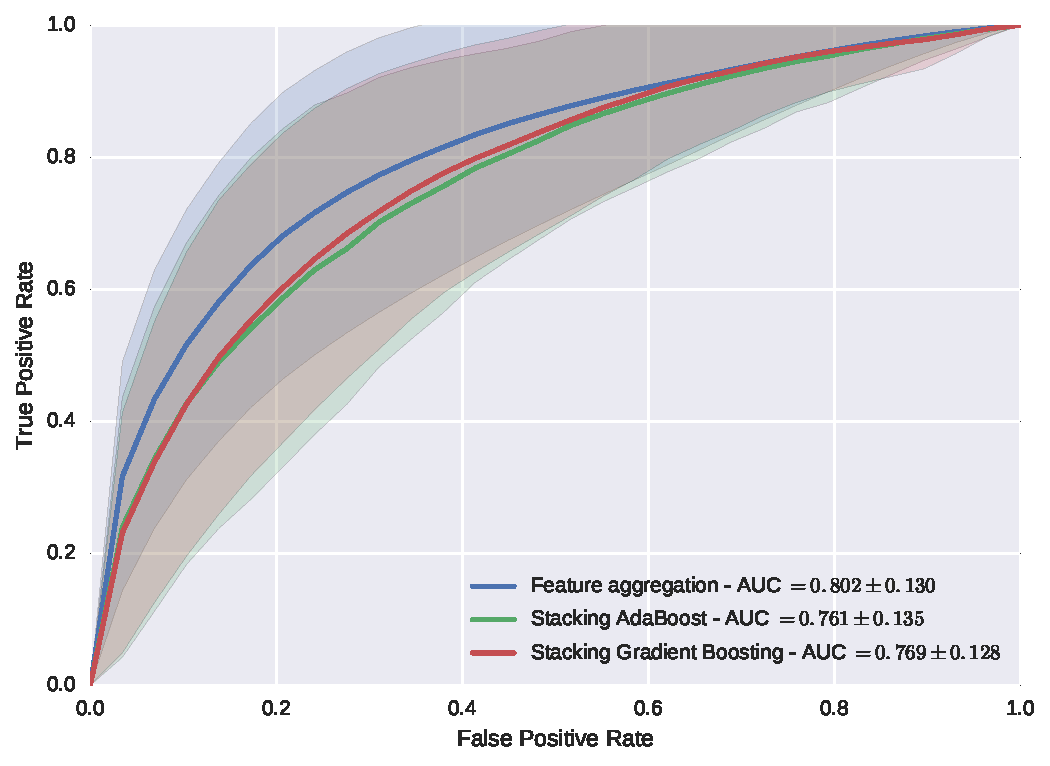
\includegraphics[width=0.7\linewidth]{6_pipeline/figures/exp-2/comb_all.pdf}
  \caption[Results obtained from experiment-2]{Results obtained from experiment-2: Coarse combination of different modaliies.}
  \label{fig:res-Exp2}
\end{figure}

\subsection{Experiment-3: Fine tuning}\label{subsec:chp6:exp-res:Ex3}
In the previous experiments (1 \& 2) the original features were used, without any adjustment or tunning. 
In this section, as we call it fine tuning, first we evaluate the performance and benefits of having a balance set, then we eavaluate different feature selection and extraction techniques.
The main aim of this experiment is to find the best balancing technique and feature selection approach suited for each modality. 
Therefore, simiar to experiment-1, only the performance of individual modalities are comapered. 

The \ac{us1} and \ac{os} techniques used to balance our training set were explained in Sect.~\ref{subsec:chp6:method:fea-bal}.
Figure~\ref{fig:res-Ex3-bal} shows the comparison of these techniques on each modality. 
\begin{figure}
  \hspace*{\fill}
  \subfigure[\ac{t2w}-\ac{mri}]{\label{fig:ex3:T2W}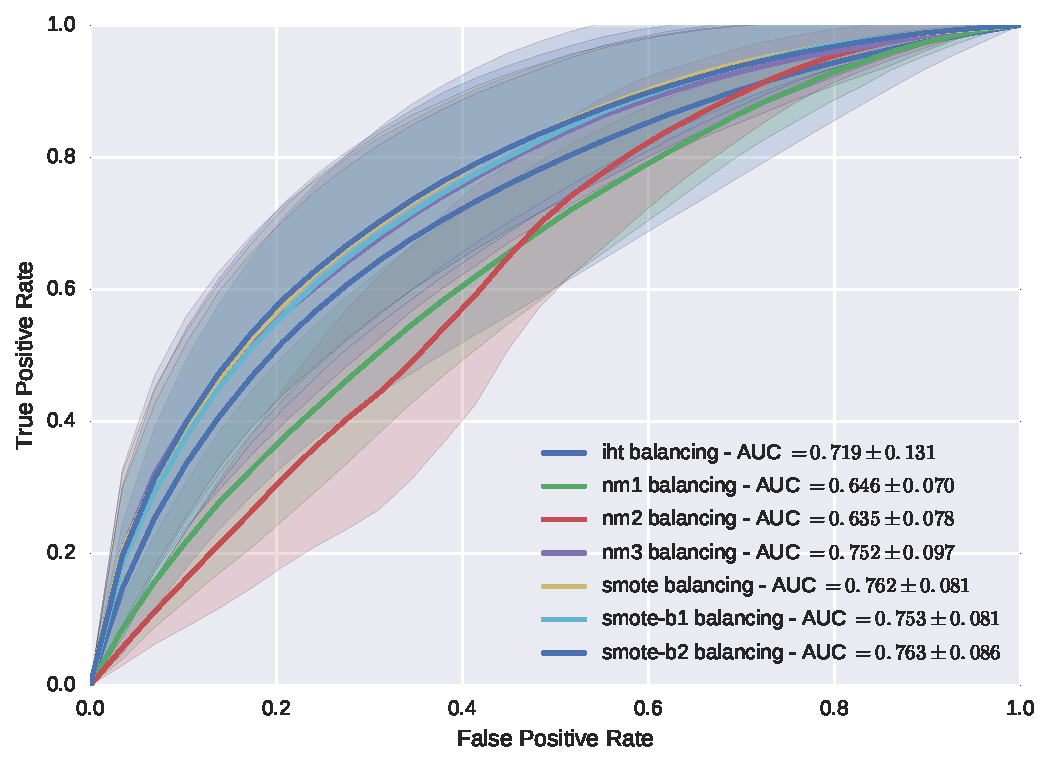
\includegraphics[width=.49\textwidth]{6_pipeline/figures/exp-3/t2w.pdf}}
  \hfill
  \subfigure[\ac{adc}-\ac{mri}]{\label{fig:ex3:ADC}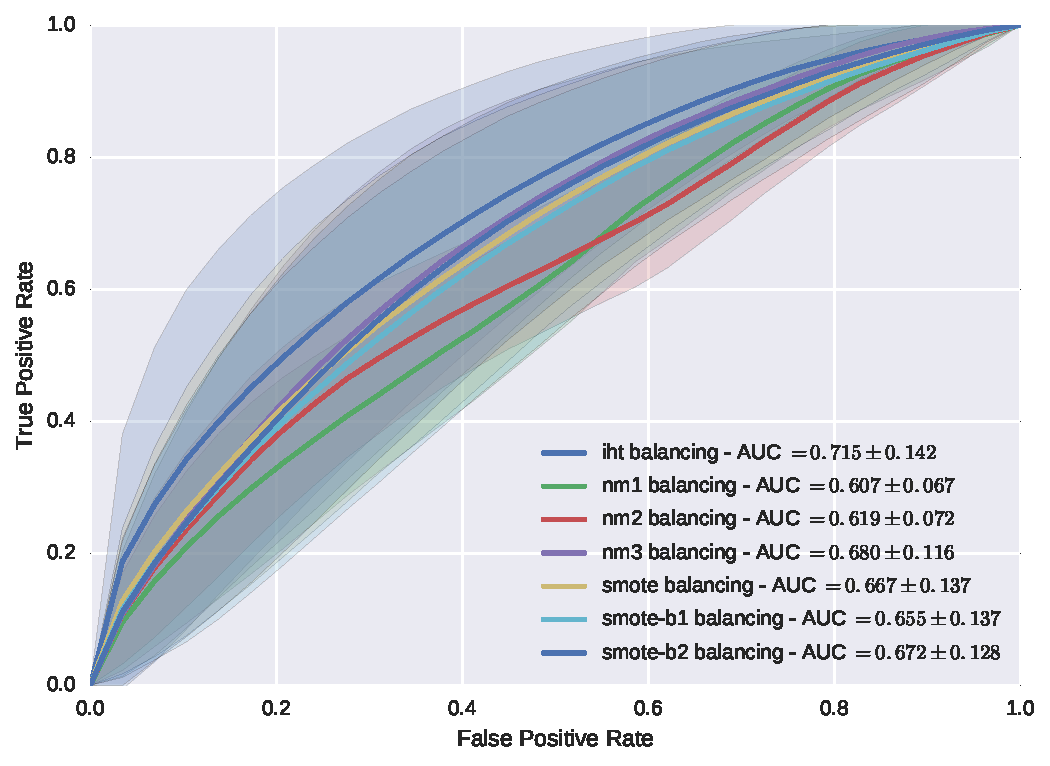
\includegraphics[width=.49\textwidth]{6_pipeline/figures/exp-3/adc.pdf}}
  \hspace*{\fill} \\
  \hspace*{\fill}
  \subfigure[\ac{dce}-\ac{mri}]{\label{fig:ex3-DCE}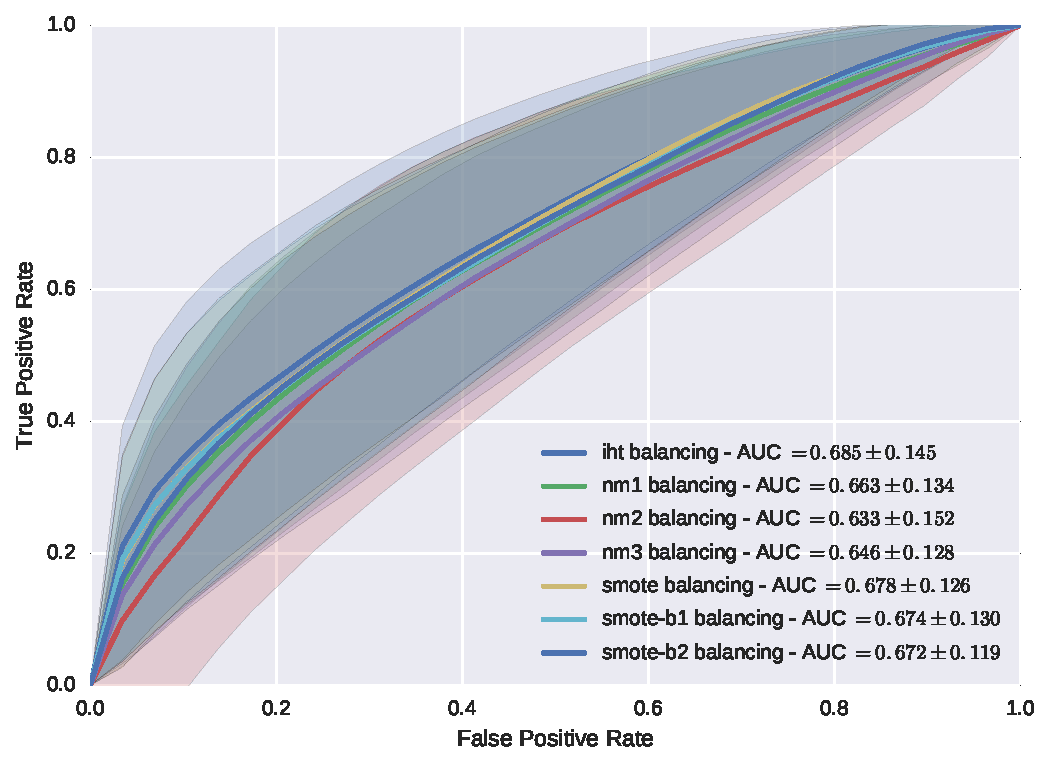
\includegraphics[width=.49\textwidth]{6_pipeline/figures/exp-3/dce.pdf}}
  \hfill
  \subfigure[\ac{mrsi}-\ac{mri}]{\label{fig:ex3-MRSI}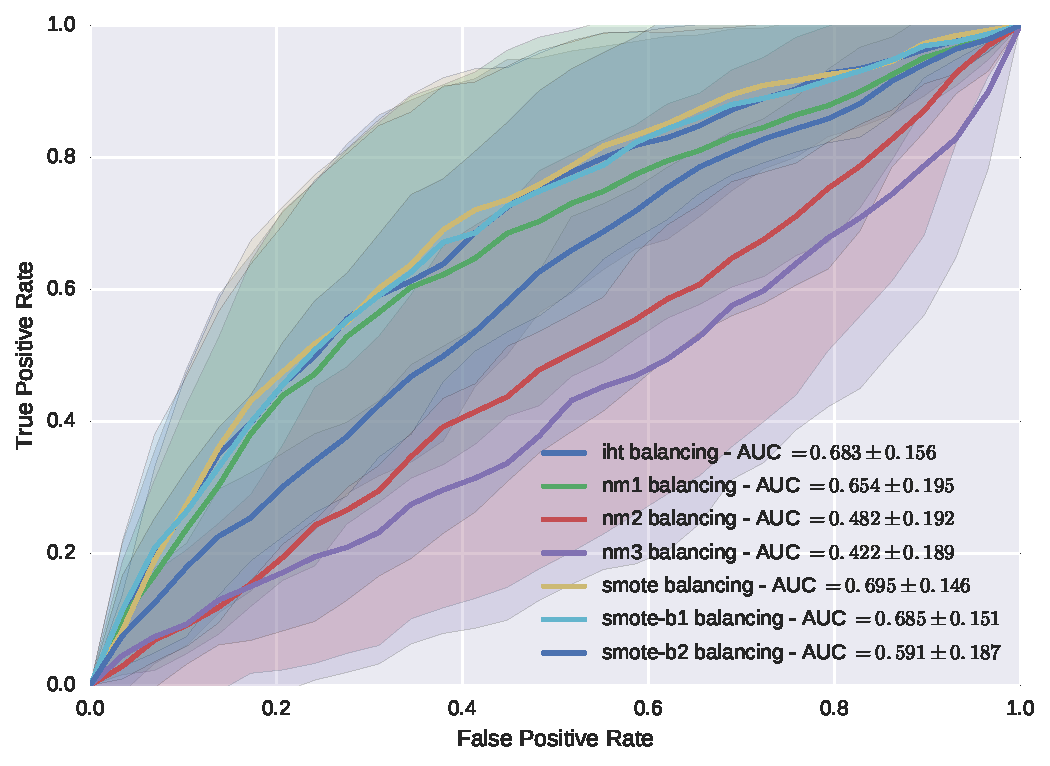
\includegraphics[width=.49\textwidth]{6_pipeline/figures/exp-3/mrsi.pdf}}
  \hspace*{\fill}
  \caption[Results obtained from experiment-3: balancing techniques.]{Results obtained from experiment-3: comparison of differnet balancing techniques on individual modalities}
  \label{fig:res-Ex3-bal}
\end{figure}

\subsection{Experiment-4: Fine combination}\label{subsec:chp6:exp-res:Ex4}
This experiments evaluates the combination of all the modalities after applying fine tunning and adjusting the feature space. 
Two different approaches are compared: (i) Feature aggregation and (ii) stacking using \ac{gb}. 
The second approach of experiment-2 was ignored, since as previously concluded, \ac{gb} had a slightly better performance than \ac{adb}.

\begin{figure}
  \centering
  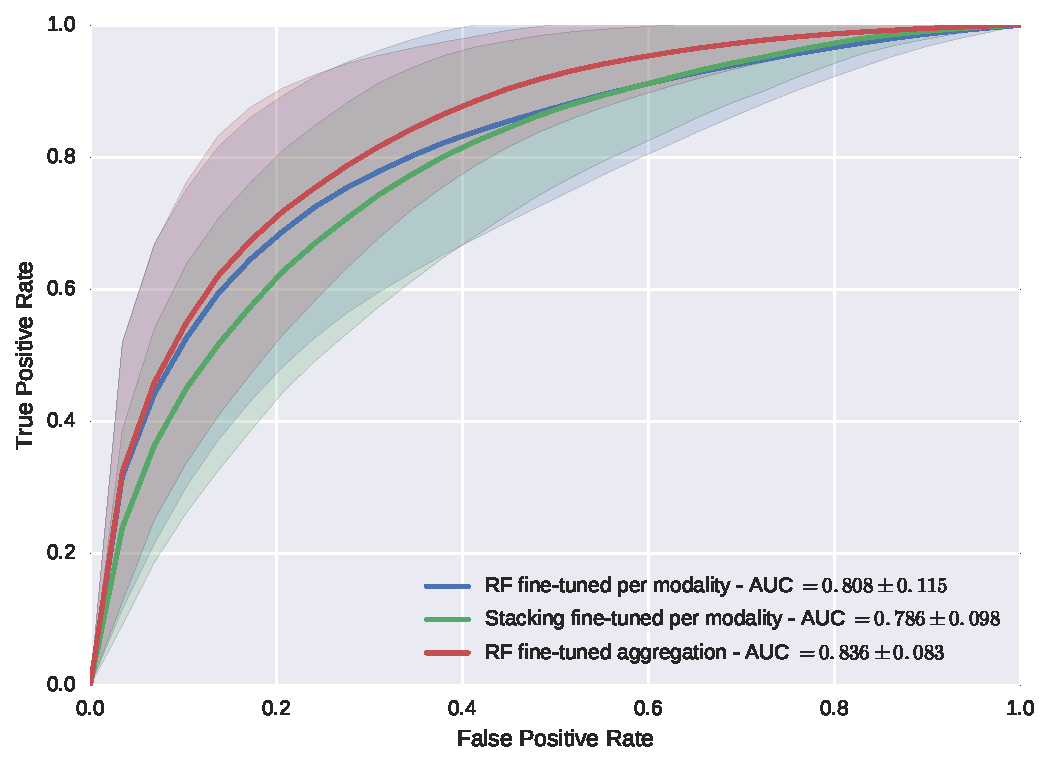
\includegraphics[width=0.7\linewidth]{6_pipeline/figures/exp-5/combine_all.pdf}
  \caption[Results obtained from experiment-4]{Results obtained from experiment-4: Fine combination of different modalities.}
  \label{fig:res-Ex4}
\end{figure}
